In this section, we describe the reduction of training data for deep learning using support vectors. As mentioned in Section 2, since deep learning requires a large amount of training data and learning time, we aim to reduce training data by extracting training data efficiently using support vectors and excluding relatively less critical data. 

\subsection{Training data reduction using support vectors}
This method reduces training data using support vectors to reduce the learning time of the neural network. Fig. 14 shows the proposed method and the learning of a conventional neural network. The procedure of the training data reduction method using support vectors is as follows. 
\begin{enumerate}
\item Train dataset $D$ with SVM and extract support vector $D_{SV}$
\item Train neural networks using $D_{SV}$ as training data
\end{enumerate}
An example of applying data reduction by support vectors to two-dimensional data is shown in Fig. 15. Focus on the following points when using support vectors.
\begin{itemize}
\item How much training data could be reduced
\item How much learning time decreased
\item What is the impact on classification accuracy
\item What happens if the same number of data is randomly extracted for the above three items
\end{itemize}
When using support vectors, if the training data is only slightly reduced, it will be meaningless. It is even more meaningless if degradation in classification accuracy occurs that does not meet the reduction in training data. Also, even if training data can be significantly reduced, classification accuracy must be maintained at a certain level. we will consider the reduction of training data while focusing on these points. However, even if we clear these conditions and confirme that only the support vectors are extracted to reduce the training data and the accuracy hardly falls, this is the undesirable result because there is no meaning using support vectors if the result is almost the same as when data reduction is performed by extracting data at random. It should be kept in mind that this may well occur if the problem to be dealt with is simple, or the training data given originally is excessive. Also, if the classification accuracy is not maintained and degraded when the support vector is used, we consider reinforcing the training data by supplementing the data not extracted as the support vector, as shown in Fig. 15(c). Since part of the data that forms the original space is supplemented, accuracy can be expected to be improved compared to when the training data is only the support vector. 
\begin{figure}[t]
  \begin{center}
  \subfigure[Reduction of training data of neural network using support vector]{
\includegraphics[width=0.8\linewidth]{fig/overview.pdf}}
\subfigure[Normal neural network learning]{
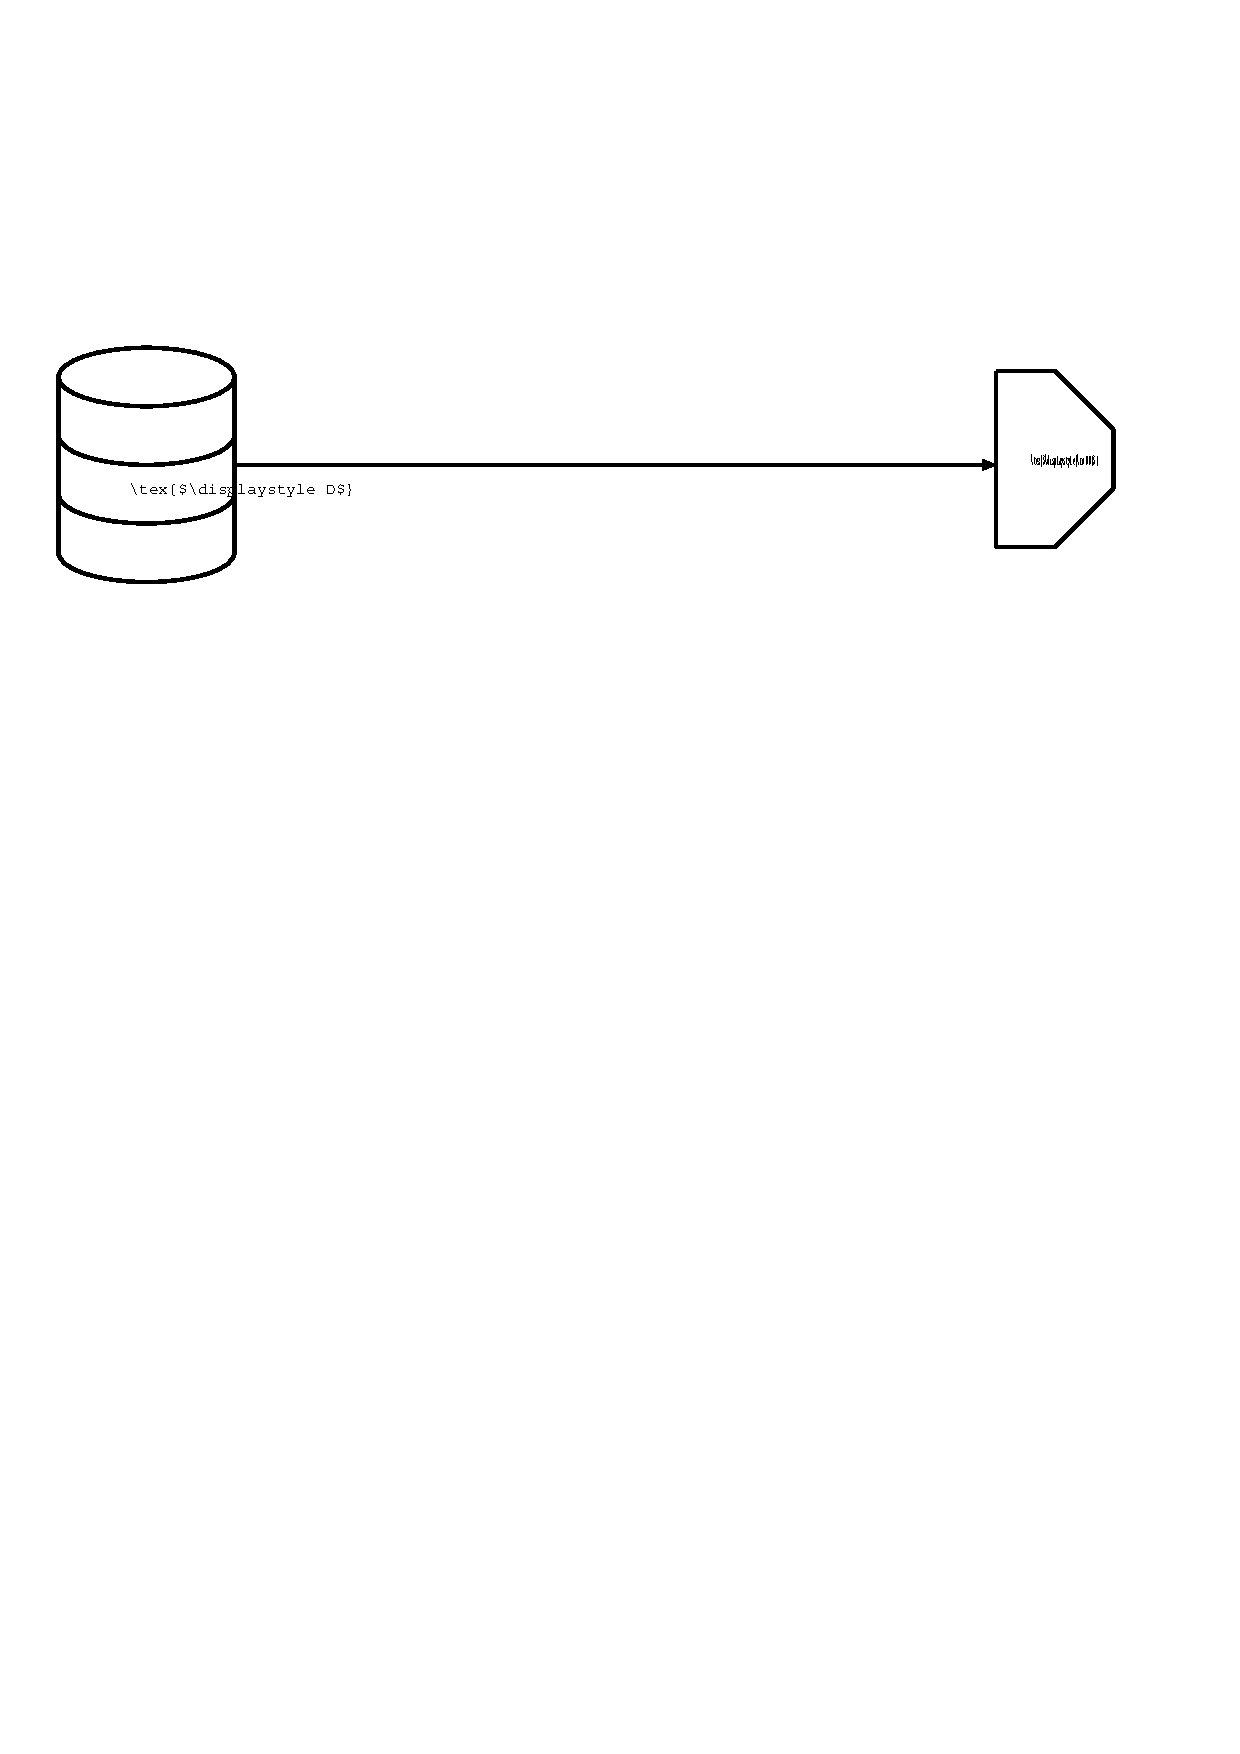
\includegraphics[width=0.8\linewidth]{fig/overview2.pdf}}
\end{center}
\caption{Reduction of training data by support vector.}
\vspace*{-3pt}
%{\hfill\footnotesize Note how the caption is centered in the column.\hfill}
\end{figure}

\begin{figure}[t]
\begin{center}
\subfigure[original data]{\includegraphics[width=0.3\linewidth]{data/C_XOR/inputdata2.png}}
\subfigure[support vector]{\includegraphics[width=0.3\linewidth]{data/C_XOR/SVMdata2.png}}
\subfigure[support vector + random]{\includegraphics[width=0.3\linewidth]{data/C_XOR/SVM+randomdata.png}}
\end{center}
\caption{Data reduction by support vector and increase of support vector by random sampling data.}
\vspace*{-3pt}
%{\hfill\footnotesize Note how the caption is centered in the column.\hfill}
\end{figure}


\subsection{Preliminary experiment}
In order to confirm the effectiveness of the training data reduction method using support vectors, we evaluate using a program with the same function as TensorFlow Playground\footnote{https://playground.tensorflow.org/} as a preliminary experiment. In the program used, two-dimensional data can be learned with a neural network, and the activation function, the number of intermediate layers, and the number of neurons can be changed arbitrarily. The two-dimensional data used in the evaluation are Gaussian (R\_GAUSS) and straight (R\_PLANE) as two types of regression problems, and Gaussian (C\_GAUSS), spiral (C\_SPIRAL), circle (C\_CIRCLE), and XOR (C\_XOR) as four types of classification problems. We evaluate the amount of data reduction and accuracy and analyze the classification results visually. In the evaluation, we used ReLU as the activation function. The middle layer is three layers, and the number of neurons in each layer is five. When we tried to reduce the data using support vectors for six types of two-dimensional data, almost no deterioration in accuracy occurred in all six. Detailed results are described in Section 4. 

In the preliminary experiment, we evaluate the classification accuracy, regression accuracy, and learning time using training data extracted by the following three methods. 
\begin{enumerate}
\item Learning using all training data
\item Learning using only support vectors
\item Learning extracting randomly as many data as support vectors
\end{enumerate}
The number of epochs is set to 100. However, because C\_SPIRAL is more complicated than the other functions and it takes time, it is set to 500 epochs. Classification accuracy is evaluated by loss, and the smaller the loss, the higher the accuracy. 

\begin{table}[b]
\begin{center}
\begin{threeparttable}
\caption{Type size for papers}
\begin{tabular}{|c|c|c|c|c|c|c|} \hline
\multirow{2}{*}{dataset} & \multicolumn{2}{|c}{(A) All training data} & \multicolumn{2}{|c}{(B) Support vector} & \multicolumn{2}{|c|}{(C)  Random} \\ \cline{2-7}

 & data & loss & data & loss & data & loss \\ \hline\hline
C\_GAUSS & 1,000 & 0.001 & 126 & 0.001 & 126 & 0.001 \\ \hline
R\_PLANE & 2,400 & 0.004 & 292 & 0.001 & 292 & 0.006 \\ \hline
R\_GAUSS & 2,400 & 0.192 & 263 & 0.011 & 263 & 0.563 \\ \hline
C\_SPIRAL & 1,000 & 0.009 & 137 & 0.039 & 137 & 0.105 \\ \hline
C\_CIRCLE & 1,000 & 0.001 & 129 & 0.002 & 129 & 0.177 \\ \hline
C\_XOR & 1,000 & 0.003 & 117 & 0.001 & 117 & 0.005 \\ \hline
\end{tabular}
%\begin{tablenotes}
%\item[a] Uppercase
%\end{tablenotes}
\end{threeparttable}
\end{center}
\end{table}


In C\_GAUSS, the accuracy was not degraded even if learning was performed using only the support vector. However, because the classification is relatively simple, even if it is randomly extracted, the accuracy is hardly degraded, and it can not be determined whether the support vector is capable. As shown in Fig. 16, although it is not classified as a clean straight line like the original data, it can be said that there is no problem because the classification itself is properly performed.

As with C\_GAUSS, R\_PLANE did not degrade in accuracy. Similarly, the effectiveness of the support vector is unknown because accuracy degradation was hardly confirmed even if it was randomly extracted. As can be seen from Fig. 17, it can be said that there is no problem as well as C\_GAUSS because all are classified in the same way.
\begin{figure}[t]
\begin{center}
\subfigure[(A) original data]{\includegraphics[width=0.40\linewidth]{data/C_GAUSS/result_099.png}}
\subfigure[(B) support vector]{\includegraphics[width=0.40\linewidth]{data/C_GAUSS/SVMresult_099.png}}
\subfigure[(C) random 1]{\includegraphics[width=0.40\linewidth]{data/C_GAUSS/Extractedresult_0.png}}
\subfigure[(C) random 2]{\includegraphics[width=0.40\linewidth]{data/C_GAUSS/Extractedresult_1.png}}
\end{center}
\caption{Evaluation in the dataset C\_GAUSS.}
\vspace*{-3pt}
%{\hfill\footnotesize Note how the caption is centered in the column.\hfill}
\end{figure}

\begin{figure}[t]
\begin{center}
\subfigure[(A) original data]{\includegraphics[width=0.40\linewidth]{data/R_PLANE/result_099.png}}
\subfigure[(B) support vector]{\includegraphics[width=0.40\linewidth]{data/R_PLANE/SVMresult_099.png}}
\subfigure[(C) random 1]{\includegraphics[width=0.40\linewidth]{data/R_PLANE/Extractedresult_0.png}}
\subfigure[(C) random 2]{\includegraphics[width=0.40\linewidth]{data/R_PLANE/Extractedresult_3.png}}
\end{center}
\caption{Evaluation in the dataset R\_PLANE.}
\vspace*{-3pt}
%{\hfill\footnotesize Note how the caption is centered in the column.\hfill}
\end{figure}
R\_GAUSS did not lose accuracy even if learning was performed using support vectors only. Besides, the accuracy was degraded in random extraction, and some did not learn well. In R\_GAUSS, a relatively complex data set, the effectiveness of the support vector was shown. Looking at Fig. 18, the support vector can be classified in the same way as the original data, so there is no problem. Also, in some cases, random classification may cause inappropriate classification.

In C\_SPIRAL, although a slight deterioration in accuracy was observed, it was not fatal and was within an acceptable range. Moreover, even if it was extracted at random, there was no significant degradation in accuracy, and it is not clear that the support vector was capable. It can be said that there is no problem because all are classified in the same way, as shown in Fig.19.
\begin{figure}[t]
\begin{center}
\subfigure[(A) original data]{\includegraphics[width=0.40\linewidth]{data/R_GAUSS/result_099.png}}
\subfigure[(B) support vector]{\includegraphics[width=0.40\linewidth]{data/R_GAUSS/SVMresult_099.png}}
\subfigure[(C) random 1]{\includegraphics[width=0.40\linewidth]{data/R_GAUSS/Extractedresult_0.png}}
\subfigure[(C) random 2]{\includegraphics[width=0.40\linewidth]{data/R_GAUSS/Extractedresult_3.png}}
\end{center}
\caption{Evaluation in the dataset R\_GAUSS.}
\vspace*{-3pt}
%{\hfill\footnotesize Note how the caption is centered in the column.\hfill}
\end{figure}
\begin{figure}[t]
\begin{center}
\subfigure[(A) original data]{\includegraphics[width=0.40\linewidth]{data/C_SPIRAL/result_499.png}}
\subfigure[(B) support vector]{\includegraphics[width=0.40\linewidth]{data/C_SPIRAL/SVMresult_499.png}}
\subfigure[(C) random 1]{\includegraphics[width=0.40\linewidth]{data/C_SPIRAL/Extractedresult_0.png}}
\subfigure[(C) random 2]{\includegraphics[width=0.40\linewidth]{data/C_SPIRAL/Extractedresult_5.png}}
\end{center}
\caption{Evaluation in the dataset C\_SPIRAL.}
\vspace*{-3pt}
%{\hfill\footnotesize Note how the caption is centered in the column.\hfill}
\end{figure}

The accuracy did not deteriorate even if C\_CIRCLE was trained only with support vectors. However, this is also relatively easy to classify, as in C\_GAUSS so even if it is randomly extracted, its accuracy is hardly degraded, and it can not be concluded that the support vector is capable. Looking at Fig. 20, although random classification sometimes resulted in somewhat angular classification, all classifications were performed without problems within the allowable range.

The accuracy did not deteriorate in the C\_XOR. Besides, even if it was randomly extracted, degradation of accuracy could hardly be confirmed, but there was a case that the classification failed considered once. Therefore, it is considered that the support vector was valid to some extent.

\begin{figure}[t]
\begin{center}
\subfigure[(A) original data]{\includegraphics[width=0.40\linewidth]{data/C_CIRCLE/result_099.png}}
\subfigure[(B) support vector]{\includegraphics[width=0.40\linewidth]{data/C_CIRCLE/SVMresult_099.png}}
\subfigure[(C) random 1]{\includegraphics[width=0.40\linewidth]{data/C_CIRCLE/Extractedresult_0.png}}
\subfigure[(C) random 2]{\includegraphics[width=0.40\linewidth]{data/C_CIRCLE/Extractedresult_6.png}}
\end{center}
\caption{Evaluation in the dataset C\_CIRCLE.}
\vspace*{-3pt}
%{\hfill\footnotesize Note how the caption is centered in the column.\hfill}
\end{figure}

\begin{figure}[t]
\begin{center}
\subfigure[(A) original data]{\includegraphics[width=0.40\linewidth]{data/C_XOR/result_099.png}}
\subfigure[(B) support vector]{\includegraphics[width=0.40\linewidth]{data/C_XOR/SVMresult_099.png}}
\subfigure[(C) random 1]{\includegraphics[width=0.40\linewidth]{data/C_XOR/Extractedresult_4.png}}
\subfigure[(C) random 2]{\includegraphics[width=0.40\linewidth]{data/C_XOR/Extractedresult_8.png}}
\end{center}
\caption{Evaluation in the dataset C\_XOR.}
\vspace*{-3pt}
%{\hfill\footnotesize Note how the caption is centered in the column.\hfill}
\end{figure}
